% !TEX root = ../stellar-notes.tex
\chapter{Binaries}\label{ch.binaries}

\section{Accretion}\label{s.accretion}

Suppose we have two objects orbiting a common center of mass.  By convention, the more massive object is known as the \emph{primary} and will be denoted by a subscript ``1''; the less massive object is the \emph{secondary} and is denoted by a subscript ``2''.  From Kepler's law, the orbital separation is
\begin{equation}\label{e.orbital-separation}
	a^{3} = G(M_{1}+M_{2}) \left(\frac{P}{2\pi}\right)^{2}, 
\end{equation}
with a numerical value $a = 0.51\nsp R_{\sun} (m_{1}+m_{2})^{1/3} (P/\hour)^{2/3}$, where we've scaled our masses to solar values, $m = M/\Msun$.

In a co-rotating frame, there is an equipotential surface with a saddle point, the \emph{inner Lagrange point}, between the two stars.  This surface forms two lobes, the \emph{Roche} lobes, that meet at this point. See the crude sketch in Figure~\ref{f.roche}.
Although the Roche lobes are not spherical, we can define the radius of an equivalent spherical volume; for the secondary, this is
\begin{equation}\label{e.r2-roche}
\frac{R_{2}}{a} \approx 0.462 \left(\frac{M_{2}}{M_{1} + M_{2}}\right)^{1/3}.
\end{equation}
As an aside, equations~(\ref{e.r2-roche}) and (\ref{e.orbital-separation}) imply that the average density of the secondary, if it fills its Roche lobe, is
\[
	\bar{\rho} = \frac{3M_{2}}{4\pi R_{2}^{3}} \approx 111\nsp\grampercc\left(\frac{\hour}{P}\right)^{2}.
\]
and does not depend explicitly on the masses of the two stars.

\begin{marginfigure}[-5\baselineskip]
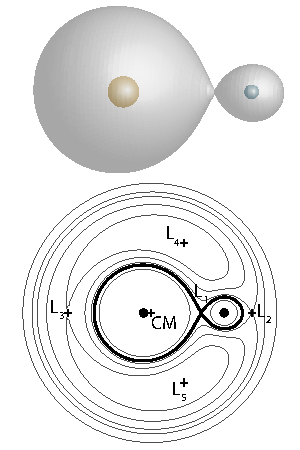
\includegraphics[width=\linewidth]{Roche}
\caption[Schematic of Roche lobes]{\label{f.roche} Sketch of the Roche lobes and potential for $M_{2} = 0.1 M_{1}$.}
\end{marginfigure}

If matter is transferred from $M_{2}$ to $M_{1}$ how does the system respond?  Let's first write down the angular momentum of the system,
\begin{equation}\label{e.roche-J}
J = (M_{1}a_{1}^{2} + M_{2}a_{2}^{2}) \omega = M_{1}M_{2}\left(\frac{Ga}{M_{1}+M_{2}}\right)^{1/2}.
\end{equation}
Here we've used equation~(\ref{e.orbital-separation}) and the relations $a_{1} = aM_{2}/(M_{1}+M_{2})$, $a_{2} = aM_{1}/(M_{1}+M_{2})$.  Let's make the assumption that no mass is lost from the system and that the mass transfer $\dot{M}$ is from $M_{2}$ to $M_{1}$:
\begin{eqnarray*}
\dot{M}_{1} + \dot{M}_{2} &=& 0;\\
\dot{M}_{2} = -\dot{M} &<& 0.
\end{eqnarray*}
Taking the logarithm of equation~(\ref{e.roche-J}) and differentiating, we then obtain
\begin{equation}\label{e.roche-adot}
\frac{\dot{a}}{a} = 2\frac{\dot{J}}{J}  + 2 \left(\frac{\dot{M}}{M_{2}}\right) \left(1-\frac{M_{2}}{M_{1}}\right).
\end{equation}
We see explicitly that for $M_{2}< M_{1}$, the response of mass transfer is to increase the orbital separation $a$ if there is no external torque on the system.

What about the size of the lobe that the secondary inhabits?  There are two countervailing tendencies: $a$ increases, which acts to increase $R_{2}$, but $M_{2}$ decreases, which acts to decrease $R_{2}$.  Taking the logarithm of eq.~(\ref{e.r2-roche}),
\begin{equation}\label{e.r2dot}
\frac{\dot{R}_{2}}{R_{2}} = \frac{\dot{a}}{a} + \frac{1}{3}\frac{\dot{M}_{2}}{M_{2}} = 2\frac{\dot{J}}{J} + 2\frac{\dot{M}}{M_{2}} \left(\frac{5}{6} - \frac{M_{2}}{M_{1}}\right).
\end{equation}
Hence for $M_{2} < (5/6) M_{1}$, the volume of the secondary's Roche lobe increases; if the secondary doesn't expand in response to mass loss and there are no external torques, then the secondary will lose contact with the inner Lagrange point and mass transfer will cease.  Alternatively, if $M_{2} > (5/6) M_{1}$, then the Roche lobe will clamp down on the secondary; this tends to drive the mass transfer at an even greater rate, and the process is unstable.

In general, there are three physical mechanisms for driving mass transfer.
\begin{description}
\item[Gravitational radiation] For $P \lesssim 2\nsp\hour$, gravitational radiation from the orbit produces a negative torque on the system:
\begin{equation}\label{e.GR-torque}
\frac{\dot{J}}{J} = -\frac{32}{5}\frac{G^{3}}{c^{5}}\frac{M_{1}M_{2}(M_{1}+M_{2})}{a^{4}}.
\end{equation}
Note that for this short of an orbital period, the binary consists of two degenerate stars (e.g., WD-WD, NS-WD).
\item[Magnetic braking] At somewhat longer periods $P \lesssim \val{1}{\unitstyle{d}}$, the companion can be a main sequence star that has a tidally locked rotation period.  Main-sequence stars have winds, and these winds carry angular momentum.  Because of the tidal locking, this also introduces a negative torque on the system.
\item[Evolution of the secondary] For wider binary orbits, the secondary star can make contact with the Roche lobe as it becomes a giant star.
\end{description}
Finally, if the secondary is sufficiently evolved, it may have a strong enough wind that accretion can still occur, even if the orbit is so wide that the secondary doesn't fill its Roche lobe.


\begin{exercisebox}[Mass-transfer from a giant]
Suppose we have a $1.6\nsp\Msun$ neutron star and a $0.8\nsp\Msun$ companion.  The companion is evolved and has an effective temperature $\Teff = 3000\nsp\K$.  We'll assume that $\Teff$ is fixed.  On the giant branch, the luminosity is powered by hydrogen shell burning, the ashes of which are added to the core (i.e., the core mass $M_{c}$ increases due to hydrogen burning).  The energy released, per gram of hydrogen consumed, is $Q = 6\ee{18}\nsp\ergs\usp\gram^{-1}$. For such an evolved giant the luminosity depends mainly on the core mass $M_{c}$ and may be approximated as \citep{Ritter1999Analytical-solu}
\[
	\frac{L}{\Lsun} = 10^{6.3}\left(\frac{M_{c}}{\Msun}\right)^{8}.
\]
For this system, find the orbital period $P$ and the mass transfer rate $\dot{M}$ (in units of solar masses per year) if the secondary has a core mass $M_{c} = 0.2\nsp\Msun$. 
\end{exercisebox}

Matter that crosses the inner Lagrange point will find itself in orbit about the primary.  The material still has enough angular momentum that it won't fall directly onto the primary, and so an \emph{accretion disk} will form. In order for the matter to accrete, there must be enough friction in the disk so that the gravitational energy can be radiated away and angular momentum transported outward.

\begin{exercisebox}[Mass-transfer due to gravitational radiation]
Suppose our binary consists of two white dwarfs with a short orbital period, less than 2 hours, so that gravitational radiation produces a torque on the system according to eq.~(\ref{e.GR-torque}).  Because the secondary is also degenerate, its radius depends on mass as
\[ R_{2} = K \left(\frac{M_{2}}{\Msun}\right)^{-1/3}, \]
where $K \approx 2\ee{9}\nsp\cm$.
\begin{enumerate}
\item Show that if the secondary just fills its Roche lobe, then $M_{2} \propto P^{-1}$ and find $M_{2}$ if $P = 1\nsp\hour$.
\item Show that
\[ \frac{\dot{M}}{M_{2}} = - \frac{\dot{J}/J}{2/3 - M_{2}/M_{1}} \]
\item Using the above relations and eq.~(\ref{e.GR-torque}), find $\dot{M}$ if $M_{1} = 1\nsp\Msun$. Scale the orbital period to units of 1 hour.
\end{enumerate}
\end{exercisebox}

\section{The Eddington Limit}

There is a characteristic luminosity at which the pressure from radiation balances the gravitational force.  This tends to act as a limit to accretion.  To derive this limit, known as the \emph{Eddington luminosity}, consider a spherically symmetric shell of matter.  Radiation enters the shell and scatters isotropically (Thomson scatters) from electrons.  The momentum flux (momentum per unit time per unit area) entering the shell is just
\[
	\bvec{P} = \frac{1}{c}\frac{L}{4\pi r^{2}} \bvec{e}_{r}.
\]
Here $L$ is the luminosity and $r$ is the radius of the shell.  Since the scattering is presumed isotropic, the rate at which the fluid element's momentum changes (the impulse imparted to it by the radiation) is just
\[
	\frac{\dif \bvec{p}}{\dif t} = \bvec{P}\sigma_{\mathrm{Th}} n_{e},
\]
where $\sigma_{\mathrm{Th}}$ is the cross-section for Thomson scattering.  Since $\dif\bvec{p}/\dif t$ is just a force per unit volume, we can balance it with the gravitational force per unit volume,
\[
\bvec{f}_{g} = -\frac{GM \langle A\rangle \mb n_{\mathrm{ion}}}{r^{2}}\bvec{e}_{r},
\]
and solve for $L$ to obtain
\begin{equation}\label{e.Ledd}
L_{\mathrm{Edd}} = \frac{4\pi GM c}{(\sigma_{\mathrm{Th}}/\mb)Y_{e}}.
\end{equation}
Here I have used $n_{e} = \langle Z\rangle n_{\mathrm{ion}}$ and $Y_{e} = \langle Z\rangle/\langle A\rangle$.
Note that $L_{\mathrm{Edd}}$ is independent of distance from the star.  Numerically,
\[ L_{\mathrm{Edd}} = 1.3\ee{38}\nsp\ergspersecond \left(\frac{M}{\Msun}\right)Y_{e}^{-1} 
	= 3.2\ee{4}\Lsun \left(\frac{M}{\Msun}\right) Y_{e}^{-1}.
\]
We can now look at what the luminosity supplied by accretion is.  First there is the just the gravitational energy release.  The gravitational release, per nucleon, is
\[ \frac{GM\mb}{R} =  \left\{\begin{array}{lr}0.069\nsp\MeV & \textrm{WD with $R=2\ee{9}\nsp\cm$}
	 \\ 138\nsp\MeV & \textrm{NS with $R = 10^{6}\nsp\cm$}\end{array}\right.
\]
In both cases we used $M = 1\nsp\Msun$.  For hydrogen-rich accretion onto a white dwarf, steady nuclear burning (assuming it exists!) will dwarf the luminosity from accretion. The situation is reversed for a neutron star, for which the energy from nuclear burning is a perturbation to the large release of gravitational binding energy.

We can compute the accretion rate at which the luminosity supplied by either nuclear burning or release of gravitational binding energy would equal the Eddington value:
\[
\dot{M}_{\mathrm{Edd}} = \left\{\begin{array}{lr}
	\frac{4\pi GM c}{Q(\sigma_{\mathrm{Th}}/\mb)Y_{e}}  & \textrm{nuclear,}\nsp L = \dot{M}Q \\
	\frac{4\pi R c}{(\sigma_{\mathrm{Th}}/\mb)Y_{e}} & \textrm{gravitational,}\nsp L= \frac{GM\dot{M}}{R}
\end{array}\right. .
\]
For nuclear burning, taking $M = 1\nsp\Msun$, $Q = 6\ee{18}\nsp\ergspergram$ (hydrogen burning), and $Y_{e} = 1$ gives $\dot{M}_{\mathrm{Edd}} = 3.3\ee{-7}\nsp\Msun\usp\yr^{-1}$.  For gravitational power, taking $R = 10^{6}\nsp\cm$ and $Y_{e} = 1$ gives $\dot{M}_{\mathrm{Edd}} = 1.5\ee{-8}\nsp\Msun\usp\yr^{-1}$.  Observed systems do in fact have inferred mass transfer rates that are typically less than these values.

\begin{exercisebox}[Energy release in the accretion disk]
\label{p.disk-L} Consider a star surrounded by an accretion disk of matter.  In the disk, which consists of ionized gas, a fluid element gradually spirals inward, so that at each point in the disk, it is approximately in a circular orbit.  Show that under these conditions, the energy radiated, per unit mass, by the fluid element over its lifetime in the disk is $GM/(2R)$.
\end{exercisebox}
